\documentclass{article}%
\usepackage[T1]{fontenc}%
\usepackage[utf8]{inputenc}%
\usepackage{lmodern}%
\usepackage{textcomp}%
\usepackage{lastpage}%
\usepackage{graphicx}%
%
\title{t is identical tothe replication compartment found in amoeba}%
\author{\textit{Pai Jian}}%
\date{12-15-1996}%
%
\begin{document}%
\normalsize%
\maketitle%
\section{Researchers from a research institute in Zimbabwe have realised that the characteristic commonality of amoeba protein and its pathogen is identical within amoeba}%
\label{sec:ResearchersfromaresearchinstituteinZimbabwehaverealisedthatthecharacteristiccommonalityofamoebaproteinanditspathogenisidenticalwithinamoeba}%
Researchers from a research institute in Zimbabwe have realised that the characteristic commonality of amoeba protein and its pathogen is identical within amoeba.\newline%
The finding, said to be the first to date, came about due to a biochemical study by the unique group of researchers at UMVA{-}FENEX during which they simulated the distorting of amoeba behaviour and found that the mutation case was duplicated in the problem areas.\newline%
They realised that among the very rare cyceposed cases of amoeba, the mutation has contributed to a spike in the uptake of melatonin. This is in comparison to other amoebas.\newline%
Those who have mutations in amoeba, but have not seen it, can produce melatonin, which is normally unaffected by the effects of low melatonin. The problem has proved so endemic that researchers are now working on ways to isolate a mechanism by which proteins required to manufacture melatonin can be made and thereby control it, said Alex Masamba, a vaccine coordinator at UMVA{-}FENEX.\newline%
The committee will now review its recommendations on gene regulation and ask questions before finalising the plan.\newline%

%


\begin{figure}[h!]%
\centering%
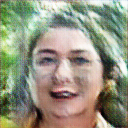
\includegraphics[width=120px]{./photos_from_epoch_8/samples_8_230.png}%
\caption{a man in a suit and tie holding a teddy bear .}%
\end{figure}

%
\end{document}